%*******************************************************
% Capitulo patrones
%*******************************************************

\chapter{Patrones}

Los patrones de diseño entregan descripciones de problemas comunes y sus soluciones tal que puedan ser reutilizados por la comunidad cada vez que se presenta el mismo problema. Un patrón describe un problema, su contexto y un esquema de solución que puede ser aplicado como plantilla.

En este capitulo se da una breve introducción a los patrones y de la sección \ref{patrones} en adelante se describe el conjunto de patrones de diseño que pueden ser aplicados en la solución.

\section{Tipos de patrones}

Los \textit{patrones de diseño} entregan descripciones de problemas comunes y sus soluciones tal que puedan ser reutilizados por la comunidad cada vez que se presenta el mismo problema. Un patrón describe un problema, su contexto y un esquema de solución que puede ser aplicado como plantilla.

Los \textit{patrones arquitectónicos} describen problemas de diseño amplios que se resuelven con transformaciones de la estructura desde una vista global.

Los \textit{patrones de datos} describen problemas recurrentes orientados a los datos y las soluciones para modelar con atributos específicos esos conjuntos de datos.

Los \textit{patrones de componentes} (también conocidos como diseño) establecen soluciones acerca de la construcción de entidades al nivel de componentes y subsistemas, y sus relaciones e interfaces.

\section{Patrones o estilos arquitectónicos}

Los patrones arquitectónicos, o patrones de arquitectura, también llamados arquetipos o estilos arquitectónicos ofrecen soluciones a problemas de arquitectura de software en ingeniería de software. Un patrón arquitectónico expresa un esquema de organización estructural esencial para un sistema de software, que consta de subsistemas, sus responsabilidades e interrelaciones. Dan una descripción de los elementos y el tipo de relación que tienen junto con un conjunto de restricciones sobre cómo pueden ser usados. En comparación con los patrones de diseño, los patrones arquitectónicos tienen un nivel de abstracción mayor.

Aunque un patrón arquitectónico comunica una imagen de un sistema, no es una arquitectura como tal. Un patrón arquitectónico es más un concepto que captura elementos esenciales de una arquitectura de software. Muchas arquitecturas diferentes pueden implementar el mismo patrón y por lo tanto compartir las mismas características o el mismo estilo. 

Uno de los aspectos más importantes de los patrones arquitectónicos es que encarnan diferentes atributos de calidad. Por ejemplo, algunos patrones representan soluciones a problemas de rendimiento y otros pueden ser utilizados con éxito en sistemas de alta disponibilidad. A primeros de la fase de diseño, un arquitecto de software escoge qué patrones arquitectónicos mejor ofrecen las calidades deseadas para el sistema.

\section{Patrones creacionales} \label{patrones}

Corresponden a patrones de diseño software que solucionan problemas de creación de instancias. Permiten encapsular y abstraer esos procesos de creación garantizando el cumplimiento de algunos atributos de calidad. Los patrones en ésta lista son \textit{Abstract factory}, \textit{Builder}, \textit{Prototype}, \textit{Singleton}.

\subsection{Abstract factory}

Este patrón permite describir la creación de familias de objetos a través de fabricas especificadas únicamente para ello.  En éste caso la creación de diferentes comentarios personalizados para las marcas es un tema que se contempla para desarrollos futuros. Debe ser posible construir diferentes tipos de comentarios para diferentes compañías y marcas. 

\begin{figure}[H]
\centering
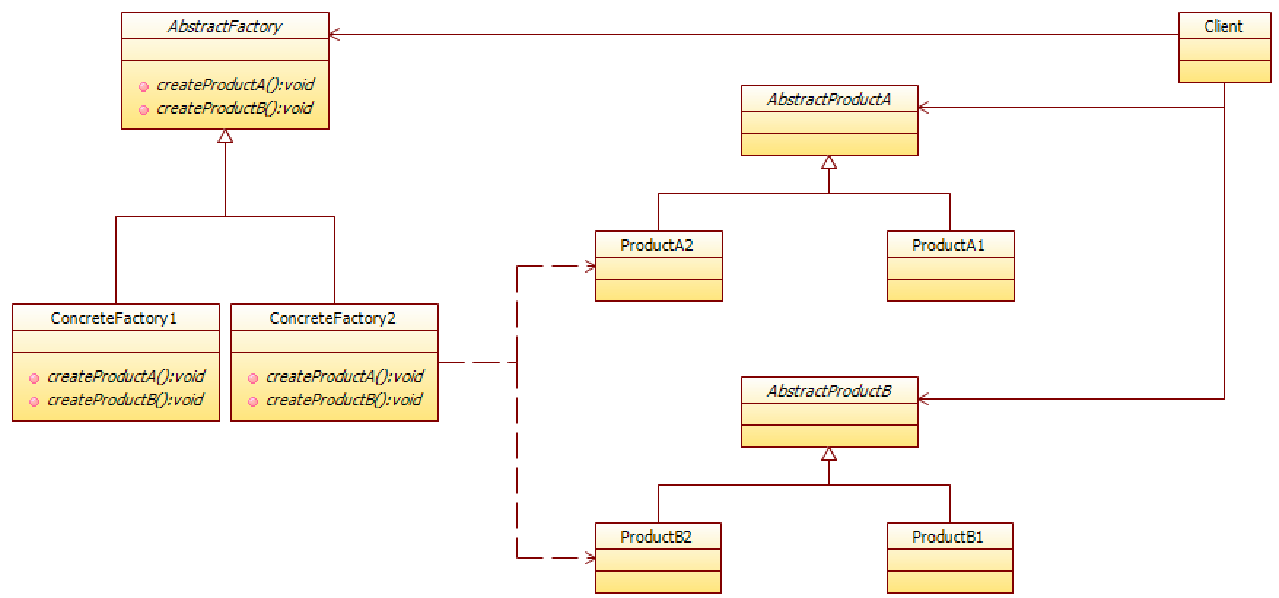
\includegraphics[scale=0.6]{Pabstractfactory}
\caption{Patrón Fábrica abstracta.}
\end{figure}

En la imagen se puede ver que hay tanto jerarquías de familias como jerarquías de fábricas. Los productos serán las diferentes configuraciones de nuevos comentarios para las marcas.  Por ejemplo, un nuevo producto podría contar con encuesta de satisfacción con una configuración de preguntas específica.

\subsection{Builder}

El patrón Builder permite la construcción automatizada de objetos complejos. Algunas de las configuraciones de marcas productos y sub-productos podría llegara a ser bastante confusa o elaborada. Se propone el uso de este patrón para construir configuraciones especiales de familias de productos con modelos de valoración independiente.  

\begin{figure}[H]
\centering
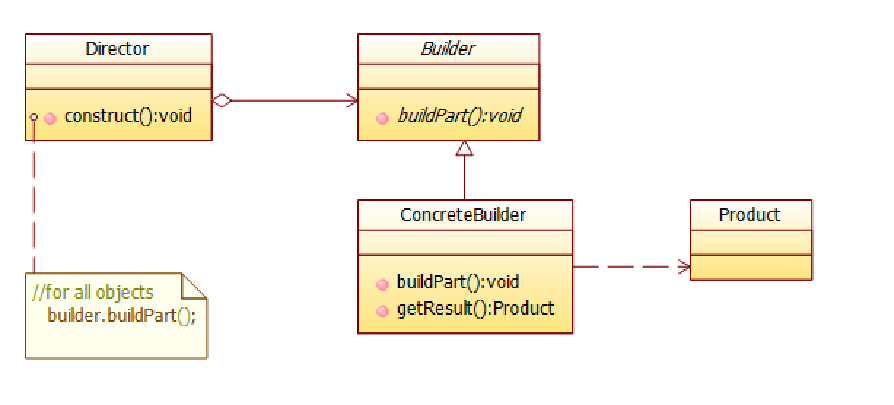
\includegraphics[scale=0.65]{Pbuilder}
\caption{Patrón Builder.}
\end{figure}

Este patrón permite a través de una clase director, que puede ser parte del cliente constructor, hacer la invocación del Builder específico (concreto) para una de las marcas específicas.   

\subsection{Prototype}

Aunque el patrón prototype es comúnmente aplicado a objetos de no son del modelo del dominio también es posible aplicarlo a los objetos de valoración compleja que sean compuestos. En el caso de los comentarios pueden tener secuencias anidadas que admitan una copia profunda.

\begin{figure}[H]
\centering
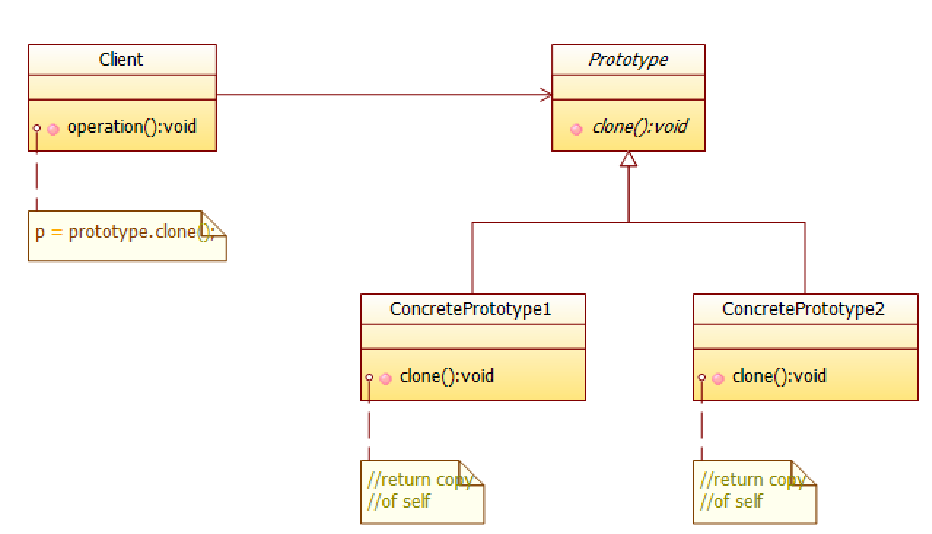
\includegraphics[scale=0.65]{Pprototype}
\caption{Patrón Pototype.}
\end{figure}

La relación de herencia también puede ser una relación de implementación de una interfaz o se puede heredar el comportamiento clone desde la clase object. 

\subsection{Singleton}

Algunos comportamientos necesarios para adminstrar el control de concurrencia y el escalamiento de la aplicación serán realizados con la clase una clase singleton que registre el comportamiento de los nuevos componentes. Cada vez que un nuevo componente sea agregado deberá existir una clase que representa el directorio de plugins registrados y ésta solo podrá tener una Instancia que será lanzada al inicio de la aplicación.

\begin{figure}[H]
\centering
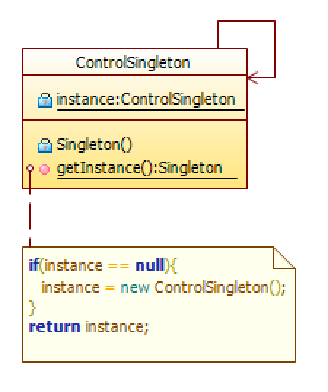
\includegraphics[scale=1.0]{Psingleton}
\caption{Patrón Singleton.}
\end{figure}


\section{Patrones estructurales}

Los patrones de diseño estructurales están enfocados en la gestión de la forma en la que las clases y los objetos se combinan para dar lugar a estructuras más complejas. Al igual que en las otros tipos de patrones, podemos hablar de patrones estructurales asociados a clases (Adapter) y asociados a objetos (Bridge, Composite, Decorator, Facade, Flyweight, Proxy). Los primeros utilizan la herencia mientras que los segundos se basan en la composición. Los patrones estructurales asociados a objetos describen formas de componer los objetos para conseguir nuevas funcionalidades. La flexibilidad de la composición de estos objetos surge de la posibilidad de cambiar dicha composición en tiempo de ejecución, lo que es imposible con la composición estática tradicional de clases.

\subsection{Adapter}

El patrón Adapter convierte la interfaz de una clase en la que otra necesita, permitiendo que clases con interfaces incompatibles trabajen juntas.

Por lo tanto, el uso de este patrón estructural está indicado cuando se quiere usar una clase ya implementada y su interfaz no es similar con la necesitada o cuando se desea crear una clase reusable que coopere con clases no relacionadas o que tengan interfaces compatibles.

\begin{figure}[H]
\centering
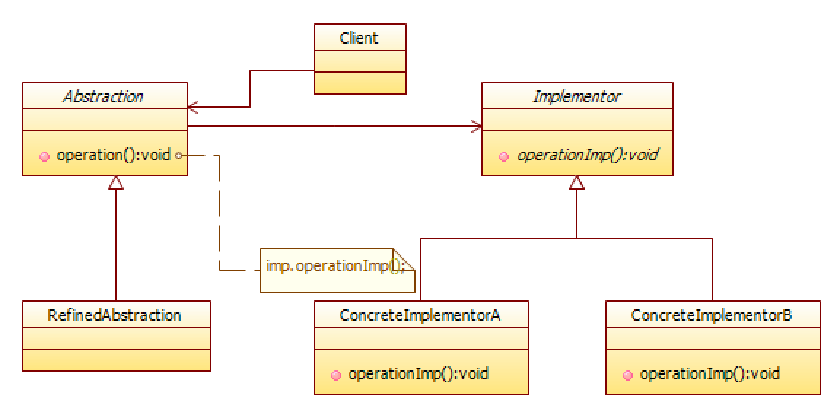
\includegraphics[scale=0.9]{Padapter}
\caption{Patrón Adapter.}
\end{figure}

Se espera que en la construcción de la aplicación todos los servicios REST funcionen como adapters en combinación con fachadas para exponer la funcionalidad de tratar a las entidades como modelos transitorios.

\subsection{Composite}

El patrón Composite sirve para construir objetos que estén formados por tros objetos más simples, pero siempre similares entre sí, gracias a la composición recursiva. Por lo tanto, al tener todos estos objetos una misma interfaz, el Composite simplifica el tratamiento de los mismos.

El patrón composite es ampliamente usado en el tratamiento de interfaces de usuario en las que se necesita, por ejemplo, representar un conjunto de elementos de una interfaz gráfica. Algunos de estos elementos serán simples, mientras que otros serán más complejos y estarán formados por varios elementos simples. Por tanto, el comportamiento y/o la información que proporciona un elemento complejo está determinada por los elementos que lo componen.
Generalizando, nos encontraríamos frente a una situación en la que necesitaríamos representar jerarquías de objetos de tipo parte y compuestos en la que se quiere usar la misma interfaz en las partes y en los compuestos. El patrón Composite, lo que nos ofrece es crear una interfaz o clase abstracta que actúe como superclase de las clases concretas que representan las partes y los compuestos. Las clases que representan los compuestos pueden ser tratadas como partes, porque soportan la interfaz.

\begin{figure}[H]
\centering
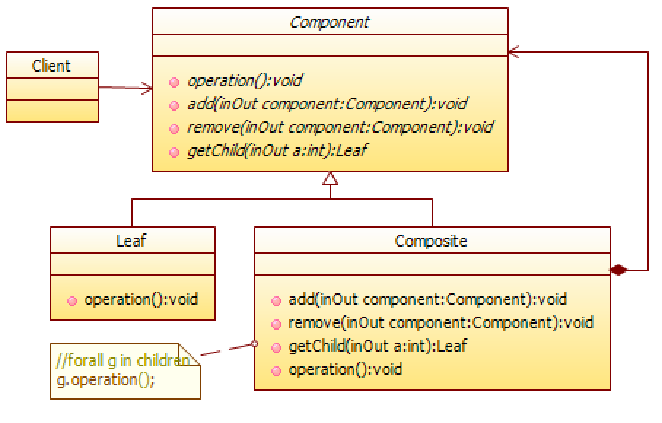
\includegraphics[scale=1]{Pcomposite}
\caption{Patrón Component.}
\end{figure}

\subsection{Decorator}

El patrón decorador permite la tarea de añadir dinámicamente funcionalidades a un Objeto. De este modo, elimina de necesidad de crear clases que fuesen heredando de la primera, incorporando no sólo la nueva funcionalidad, sino también otras nuevas y asociarlas a ella.

A veces se desea adicionar responsabilidades a un objeto pero no a toda la clase. Las responsabilidades se pueden adicionar por medio de los mecanismos de Herencia, pero este mecanismo no es flexible porque la responsabilidad es adicionada estáticamente. La solución flexible es la de rodear el objeto con otro objeto que es el que adiciona la nueva responsabilidad. Este nuevo objeto es el Decorator.

Este ejemplo de diseño  es útil cuando:
\begin{itemize}
    \item Se quiere añadir o expander las funcionalidades de objetos de forma dinámica y transparente. Con éste se logra escalar las funcionalidades a nuevas plateas rapidamente.
 \item Necesitamos que ciertas responsabilidades de un objeto puedan ser retiradas de forma sencilla en un futuro.
 \item No es posible o no compensa realizar esta expansión de funcionalidades mediante herencia.
 \item Existe la necesidad de expandir dinámicamente la funcionalidad de un objeto y/o eliminar la funcionalidad extendida.
\end{itemize}

\begin{figure}[H]
\centering
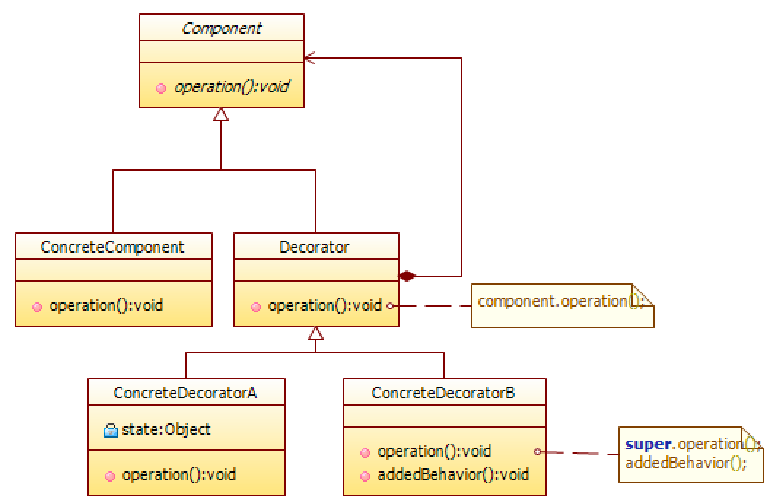
\includegraphics[scale=0.9]{Pdecorator}
\caption{Patrón decorador.}
\end{figure}


\subsection{Facade}

Provee una interfaz unificada para un grupo de interfaces en un subsistema, de manera que esta funcione como una interfaz de alto nivel que hace al resto de las interfaces fácil de usar.

\begin{figure}[H]
\centering
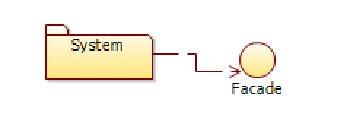
\includegraphics[scale=1.0]{Pfacade}
\caption{Patrón fachada.}
\end{figure}

Todos los servicios REST que serán creados estarán bajo la implementación de Facade.

\subsection{Flyweight}

El patrón Flyweight (u objeto ligero) sirve para eliminar o reducir la redundancia cuando tenemos gran cantidad de objetos que contienen información idéntica, además de lograr un equilibrio entre flexibilidad y rendimiento (uso de recursos).

\begin{figure}[H]
\centering
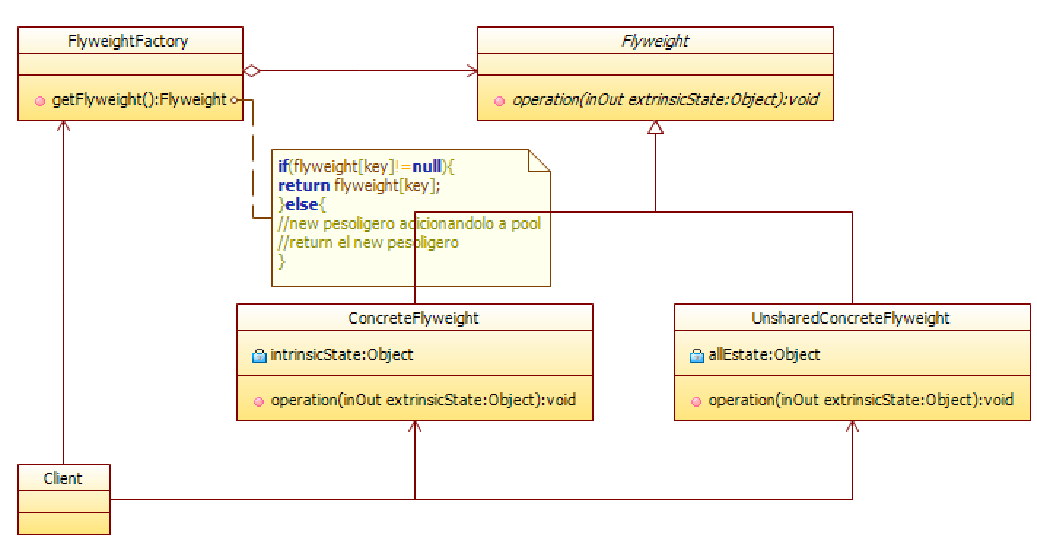
\includegraphics[scale=0.7]{Pflyweight}
\caption{Patrón flyweight.}
\end{figure}

\subsection{Proxy}

La finalidad principal del patrón de diseño estructural Proxy, es proporcionar un representante o sustituto de otro objeto para controlar el acceso a éste. Esto lo hace según la motivación de retrasar el costo de crear e inicializar un objeto hasta que sea realmente necesario. Por lo tanto, es usado cuando se necesita una referencia a un objeto más flexible o sofisticado que una referencia. Por ejemplo, si que queremos construir una aplicación que usa muchos objetos visuales, lo ideal es que dichos objetos sólo se instanciaran cuando se vayan a utilizar, de tal forma que se ahorre carga en memoria y tiempo.

\begin{figure}[H]
\centering
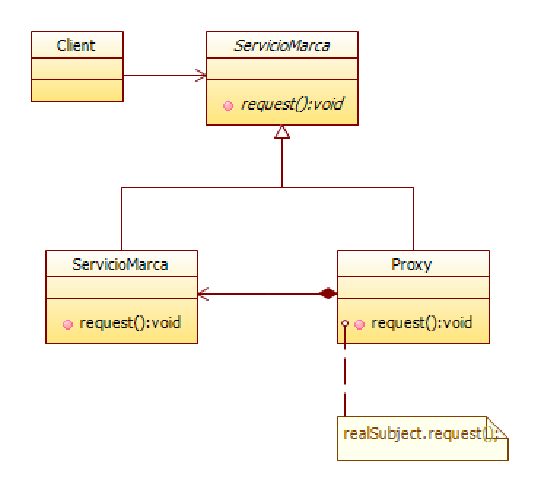
\includegraphics[scale=0.8]{Pproxy}
\caption{Patrón proxy.}
\end{figure}

Lo mismo ocurre cuando en el modelo de administración de persistencia debemos instanciar objetos o mantener en cache algunos otros que no sean persistentes.

\section{Patrones de comportamiento}

Los patrones de diseño software de comportamiento son aquellos que están relacionados con algoritmos y con la asignación de responsabilidades a los objetos.
Describen no solamente patrones de objetos o de clases, sino que también engloban patrones de comunicación entre ellos. Al igual que los otros tipos de patrones, se pueden clasificar en función de que trabajen con clases (Template Method, Interpreter) u objetos (Chain of Responsability, Command, Iterator, Mediator, Memento, Observer, State, Strategy, Visitor).

La variación de la encapsulación es la base de muchos patrones de comportamiento. Cuando un aspecto de un programa cambia frecuentemente, estos patrones trabajan con un objeto que encapsula dicho aspecto, teniendo que definir por tanto, una clase abstracta que describe la encapsulación del objeto.

\subsection{Chain of responsability}

Es un patrón de comportamiento que evita acoplar el origen de una petición a su receptor dando a más de un objeto la posibilidad de responder a una petición. Para ello, se encadenan los receptores y pasa la petición a través de la cadena hasta que es procesada por algún objeto. Este patrón es utilizado a menudo en el contexto de las interfaces gráficas de usuario donde un objeto puede estar compuesto de varios objetos (que generalmente heredán de una super clase "vista").

\begin{figure}[H]
\centering
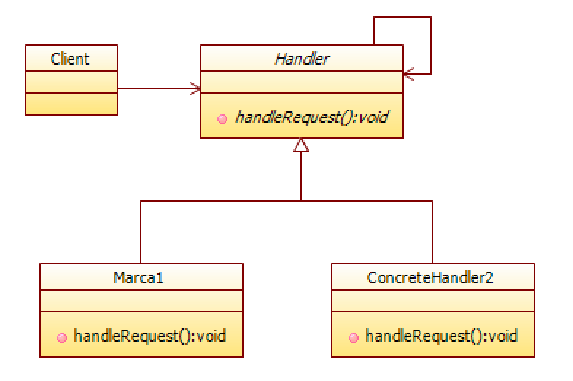
\includegraphics[scale=0.9]{Pchainresponsability}
\caption{Patrón cadena de responsabilidad.}
\end{figure}

En este caso existe una cadena de mensajes en los comentarios de la marca y una cadena de publicación que son una serie de personas que autorizan o no la publicación de diferentes comentarios.

\subsection{Command}

El patrón de diseño software de comportamiento Command permite realizar una operación sobre un objeto sin conocer realmente las instrucciones de esta operación ni el receptor real de la misma. Esto se consigue encapsulando la petición como si fuera un objeto, con lo que además se facilita la parametrización de los métodos.

\begin{figure}[H]
\centering
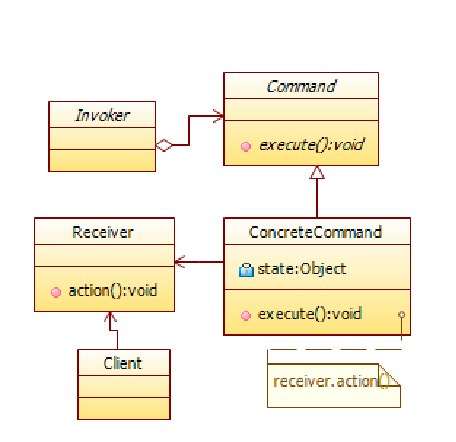
\includegraphics[scale=1.0]{Pcomando}
\caption{Patrón Comando.}
\end{figure}

\subsection{State}

En determinadas ocasiones, cuando el contexto en el que se está desarrollando requiere que un objeto tenga diferentes comportamientos según el estado en que se encuentra, resulta complicado poder manejar el cambio de comportamientos y los estados de dicho objeto, todos dentro del mismo bloque de código. El patrón State propone una solución a esta complicación, creando básicamente, un objeto por cada estado posible del objeto que lo llama. Permite a un objeto alterar su comportamiento según el estado interno en que se encuentre.

Existe una extrema complejidad en el código cuando se intenta administrar comportamientos diferentes según una cantidad de estados diferentes. Asimismo el mantenimiento de este código se torna difícil, e incluso se puede llegar en algunos casos puntuales a la incongruencia de estados actuales por la forma de implementación de los diferentes estados en el código (por ejemplo con variables para cada estado).

\begin{figure}[H]
\centering
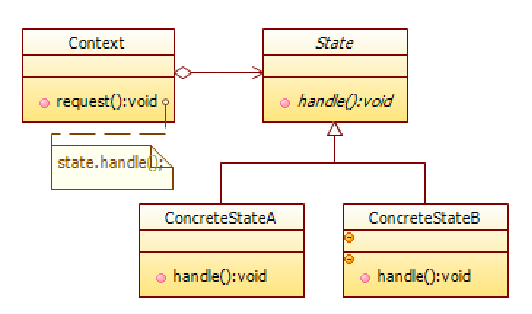
\includegraphics[scale=1.0]{Pstate}
\caption{Patrón State.}
\end{figure}

\subsection{Strategy}

Este es un patrón de diseño software de comportamiento que determina la forma de implementar el intercambio de mensajes entre diferentes objetos que realizan diferentes tareas, pero que comparten elementos comunes. El patrón de comportamiento Strategy permite gestionar un conjunto de operaciones de entre los cuales el cliente puede elegir el que le convenga más en cada situación, e intercambiarlo, de forma dinámica, cuando lo necesite.

Para llevar a cabo esta funcionalidad, este patrón de comportamiento trabaja con los algoritmos que implementan las diferentes estrategias de forma que los encapsula en una jerarquía, consiguiendo que el cliente trabaje contra un objeto intermediario o 'Context'. En este punto, el cliente puede elegir el algoritmo que prefiera de entre los implementados en las estrategias del sistema, o dejar al contexto la tarea de elegir al más apropiado para cada situación concreta.
Por lo tanto, cualquier sistema que presente un servicio o función determinada, que pueda o deba ser realizada de varias maneras dependiendo del contexto, será indicado gestionarlo con el patrón Strategy.

\begin{figure}[H]
\centering
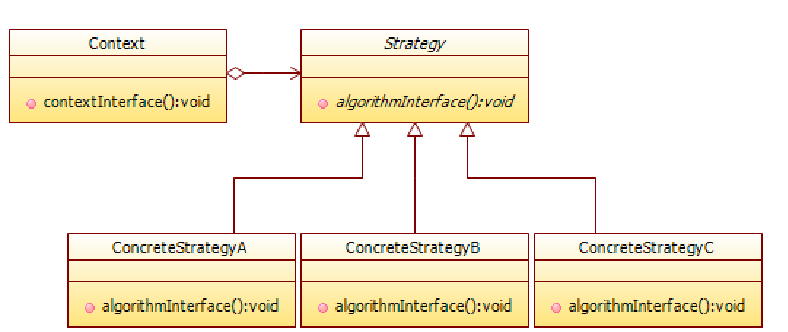
\includegraphics[scale=0.8]{Pstrategy}
\caption{Patrón Strategy.}
\end{figure}

\subsection{Interpreter}

El interpreter es un patrón de diseño que, dado un lenguaje, define una representación para su gramática junto con un intérprete del lenguaje.

Se usa para definir un lenguaje para representar expresiones regulares que representen cadenas a buscar dentro de otras cadenas. Además, en general, para definir un lenguaje que permita representar las distintas instancias de una familia de problemas.

Se requiere para hacer análisis gramatical en la aplicación y determinar palabras clave en los comentarios.

\begin{figure}[H]
\centering
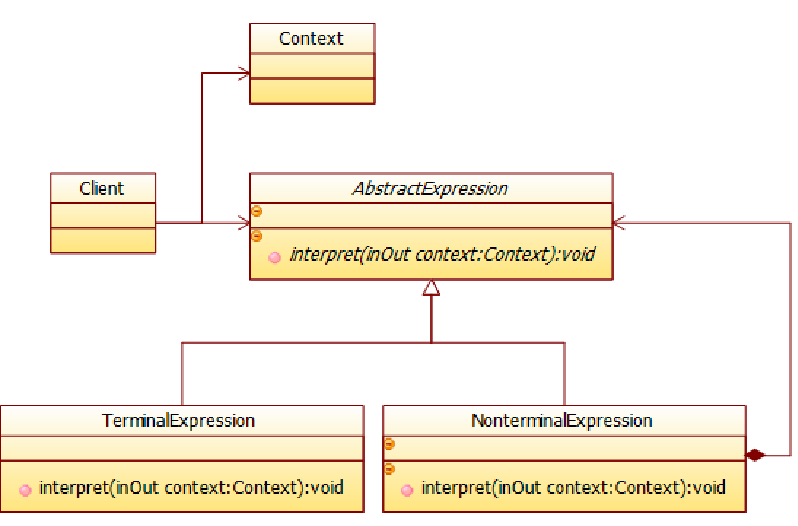
\includegraphics[scale=0.8]{Pinterpreter}
\caption{Patrón Interprete.}
\end{figure}

\subsection{Iterator}

El patrón de diseño de comportamiento Iterator es uno de los mayores exponentes de los patrones de comportamient. Presenta la interfaz que declara los métodos necesarios para acceder, de forma secuencial, a los objetos de una colección.

El iterator cubre la necesidad de acceder a los elementos de un contenedor de objetos sin tener que trabajar con su estructura interna. Además, es posible que se necesite más de una forma de recorrer la estructura siendo para ello necesario crear modificaciones en la clase. Mediante el uso del patrón, se añaden métodos que permiten recorrerla sin referenciar su representación, por lo que la responsabilidad del recorrido se traslada a un objeto iterador.

La gran desventaja de que usar este objeto iterador, más o menos encapsulado, es que muchas veces se necesita conocer la estructura del contenedor para elegir del tipo de iterador más adecuado. Esto se soluciona abstrayendo los tipos de los distintos iteradores y dotando a las estructuras de un método que cree un iterador concreto.

\begin{figure}[H]
\centering
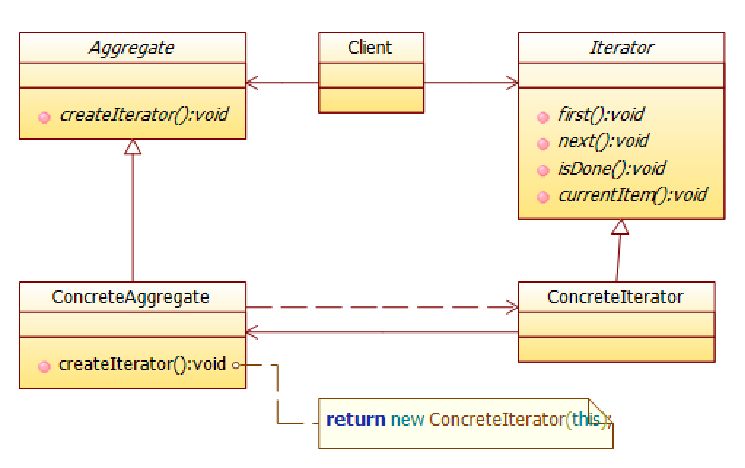
\includegraphics[scale=0.7]{Piterator}
\caption{Patrón Iterador.}
\end{figure}

\subsection{Mediator}

El patrón mediador define un objeto que encapsula cómo un conjunto de objetos interactúan. Este patrón de diseño está considerado como un patrón de comportamiento debido al hecho de que puede alterar el comportamiento del programa en ejecución.

Habitualmente un programa está compuesto de un número de clases (muchas veces elevado). La lógica y computación es distribuida entre esas clases. Sin embargo, cuantas más clases son desarrolladas en un programa, especialmente durante mantenimiento y/o refactorización, el problema de comunicación entre estas clases quizás llegue a ser más complejo. Esto hace que el programa sea más difícil de leer y mantener. Además, puede llegar a ser difícil cambiar el programa, ya que cualquier cambio podría afectar código en muchas otras clases.

Con el patrón mediador, la comunicación entre objetos es encapsulada con un objeto mediador. Los objetos no se comunican de forma directa entre ellos, en lugar de ello se comunican mediante el mediador. Esto reduce las dependencias entre los objetos en comunicación, reduciendo entonces la Dependencia de código.


\begin{figure}[H]
\centering
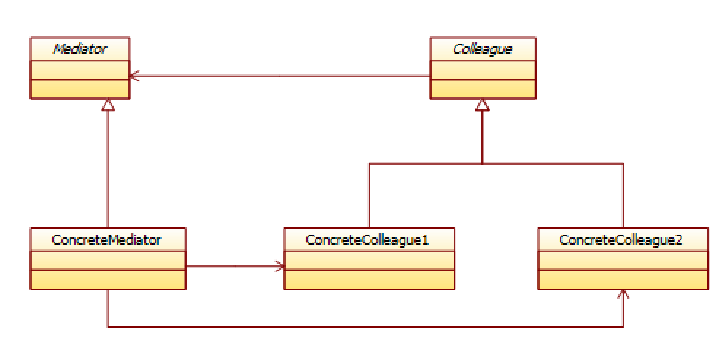
\includegraphics[scale=1]{Pmediator}
\caption{Patrón Mediador.}
\end{figure}

\subsection{TemplateMethod}

El método de template está diseñado para marcos, donde cada cual implementa las partes invariables de la arquitectura de un ámbito, dejando "placeholders" para personalizar las opciones. Esto es un ejemplo de inversión de control. Alguna razones por la que se utiliza el método de plantilla son:

Dejar que las subclases que se implementan (a través del método primordial) tengan un comportamiento que puede variar.

Evitar duplicación en el código: la estructura general de flujo de trabajo, está implementada una vez en el algoritmo de clase abstracta, y variaciones necesarias son implementadas en cada de las subclases.

Control en qué punto(s) la subclassing está permitida. En oposición a una sencilla sobrecarga polimórfica, donde el método de base sería enteramente reescrito, permitiendo un cambio radical en el flujo. Sólo los detalles específicos del flujo se pueden cambiar.

\begin{figure}[H]
\centering
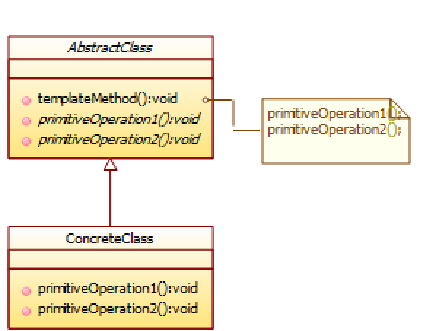
\includegraphics[scale=0.8]{Ptemplatemethod}
\caption{Patrón Template Method.}
\end{figure}

\subsection{Memento}

Memento es un patrón cuya finalidad es almacenar el estado de un objeto (o del sistema completo) en un momento dado de manera que se pueda restaurar en ese punto de manera sencilla, además sirve para facilitar a la gente floja realizar los programas. Para ello se mantiene almacenado el estado del objeto para un instante de tiempo en una clase independiente de aquella a la que pertenece el objeto (pero sin romper la encapsulación), de forma que ese recuerdo permita que el objeto sea modificado y pueda volver a su estado anterior. Aunque suele ser poco pertinente para su uso.

\begin{figure}[H]
\centering
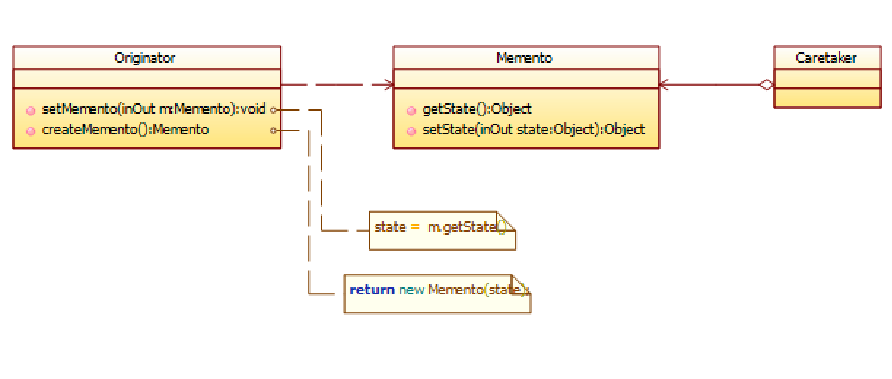
\includegraphics[scale=0.9]{Pmemento}
\caption{Patrón Memento.}
\end{figure}

\subsection{Observer}

El patrón de comportamiento Observer define una interacción entre objetos, de manera que cuando uno de ellos cambia su estado, el Observer se encarga de notificar este cambio a los demás.

Por tanto, la razón de ser de este patrón es desacoplar las clases de los objetos, aumentando la modularidad del lenguaje y evitando bucles de actualización.

La idea básica del patrón es que el objeto de datos (o sujeto) contenga atributos mediante los cuales cualquier objeto observador (o vista) se pueda suscribir a él pasándole una referencia a sí mismo. De este modo, el sujeto mantiene así una lista de las referencias a sus observadores.

Dadas estas propiedades, el patrón Observer suele emplearse en el desarrollo de frameworks de interfaces gráficas orientados a objetos, enlazando 'listeners' a los objetos que pueden disparar eventos.

\begin{figure}[H]
\centering
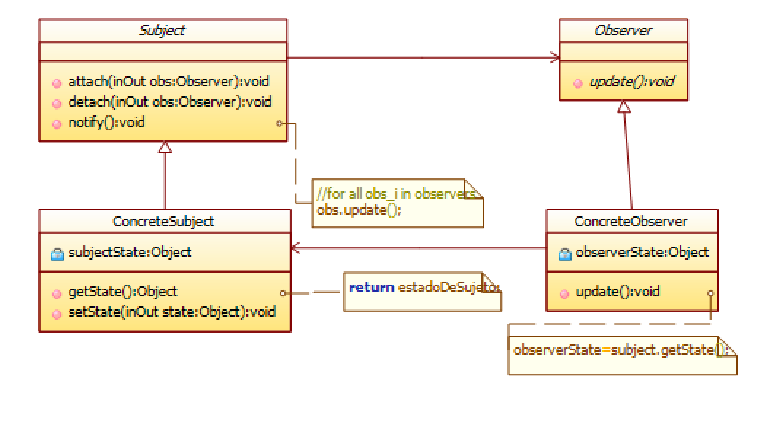
\includegraphics[scale=0.8]{Pobserver}
\caption{Patrón Observador.}
\end{figure}

\subsection{Visitor}

La idea básica es que se tiene un conjunto de clases elemento que conforman la estructura de un objeto. Cada una de estas clases elemento tiene un método aceptar (accept()) que recibe al objeto visitante (visitor) como argumento. El visitante es una interfaz que tiene un método visit diferente para cada clase elemento; por tanto habrá implementaciones de la interfaz visitor de la forma: visitorClase1, visitorClase2... visitorClaseN. El método accept de una clase elemento llama al método visit de su clase. Clases concretas de un visitante pueden entonces ser escritas para hacer una operación en particular.

\begin{figure}[H]
\centering
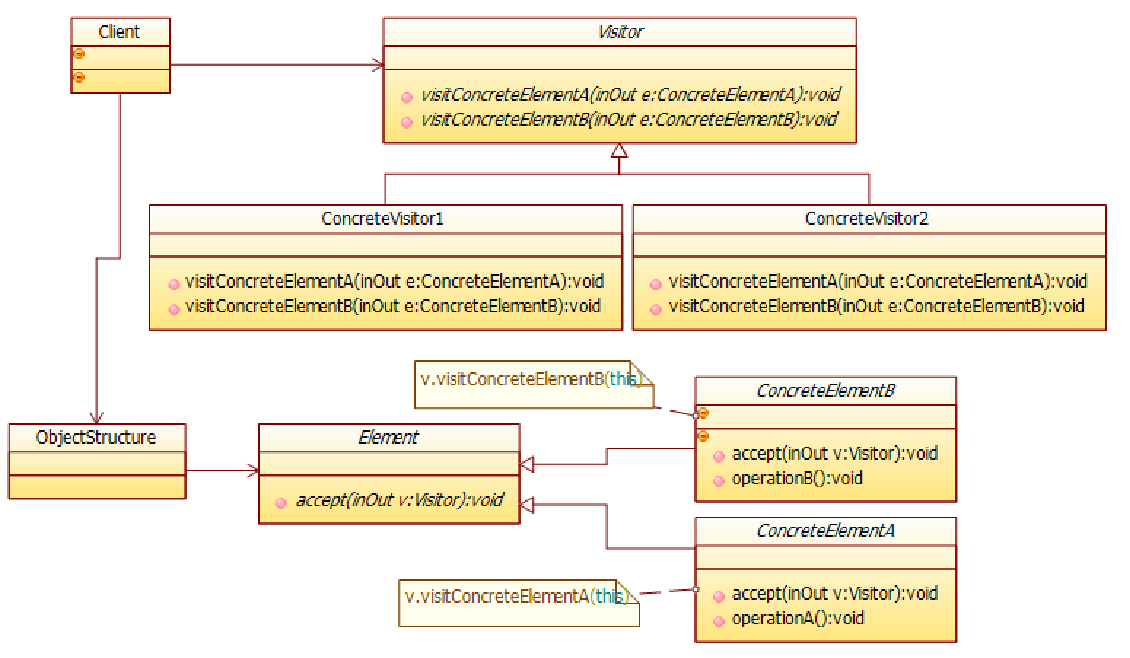
\includegraphics[scale=0.6]{Pvisitor}
\caption{Patrón Visitador.}
\end{figure}